% This is samplepaper.tex, a sample chapter demonstrating the
% LLNCS macro package for Springer Computer Science proceedings;
% Version 2.20 of 2017/10/04
%
\documentclass[runningheads]{llncs}
%
\usepackage{graphicx}
\usepackage{multirow} 
\usepackage{fancyvrb}
\usepackage[misc,geometry]{ifsym} 


% Used for displaying a sample figure. If possible, figure files should
% be included in EPS format.
%
% If you use the hyperref package, please uncomment the following line
% to display URLs in blue roman font according to Springer's eBook style:
% \renewcommand\UrlFont{\color{blue}\rmfamily}

\begin{document}
%
\title{ON SECONDARY STRUCTURE ANALYSIS BY USING FORMAL GRAMMARS AND ARTIFICIAL NEURAL NETWORKS\thanks{Supported by the Russian Science Foundation grant 18-11-00100}}
%
\titlerunning{Formal Grammars \& Neural Networks}
% If the paper title is too long for the running head, you can set
% an abbreviated paper title here
%
\author{Polina Lunina\inst{1,2}\orcidID{0000-0002-7172-2647} \Letter \and
Semyon Grigorev\inst{1,2}\orcidID{0000-0002-7966-0698}}
%
\authorrunning{Polina Lunina, Semyon Grigorev}
% First names are abbreviated in the running head.
% If there are more than two authors, 'et al.' is used.
%
\institute{Saint Petersburg State University, 7/9 Universitetskaya nab., St. Petersburg, 199034, Russia \and
JetBrains Research, Primorskiy prospekt 68-70, Building 1, St. Petersburg 197374, Russia\\
\email{lunina\_polina@mail.ru \Letter, semyon.grigorev@jetbrains.com, s.v.grigoriev@spbu.ru}\\
}
%
\maketitle              % typeset the header of the contribution
%
\begin{abstract}
A way to combine formal grammars and artificial neural networks for biological sequences processing was recently proposed.
In this approach, an ordinary grammar encodes primitive features of the RNA secondary structure, parsing is utilized for features extraction and artificial neural network~--- for processing of the extracted features.
Parsing is a bottleneck of the solution: input sequences should first be parsed before processing with a trained model which is a time-consuming operation when working with huge biological databases.
In this work, we solve this problem by employing staged learning and limiting parsing to be used only during network training.
We also compare networks which represent the parsing result in two different ways: by a vector and a bitmap image.
Finally, we evaluate our solution on tRNA classification tasks.

\keywords{DNN \and CNN \and Machine Learning \and Secondary Structure \and Genomic Sequences \and Formal Grammars \and Parsing.}
\end{abstract}
%
%
%

\section{Introduction}

Foundation in some areas: graphs, code analysis, etc.
Why is it important to proof B-H in Coq?
Bar-Hillel theorem is a main on �.
Short overview of current results.

\section{Ordinary Context-Free Grammars and Artificial Neural Networks for Secondary Structure Analysis}

In this section we provide a brief description of the approach for the genomic sequences secondary structure analysis which is proposed in~\cite{grigorevcomposition}.

The secondary structure of RNA sequences can be viewed as a composition of stems~\cite{MQbioinformatics19}.
Grammar $G_0$ that is used in~\cite{grigorevcomposition} as well as in the present work is presented in figure~\ref{gram}.
This grammar considers only the conventional base pairs (line \textbf{5}) and describes the recursive composition of stems which are at least three base pairs in height (lines \textbf{7-12}).
Stems may be connected by an arbitrary sequence of length from 2 up to 10, and loops also have length from 2 up to 10 (line \textbf{2}).
These parameters were tuned manually as a result of the number of experiments and can be changed to provide a better grammar for some specific goal.

\begin{figure}
\begin{Verbatim}[numbers=left,xleftmargin=5mm]
s1: stem<s0>
any_str : any_smb*[2..10]
s0: any_str | any_str stem<s0> s0
any_smb: A | U | C | G
stem1<s>: A s U | G s C | U s A | C s G 
stem2<s>: stem1< stem1<s> >
stem<s>:  
      A stem<s> U 
    | U stem<s> A 
    | C stem<s> G 
    | G stem<s> C 
    | stem1< stem2<s> >  
\end{Verbatim}
\caption{Context-free grammar $G_0$ for RNA secondary structure features description}
\label{gram}
\end{figure}

The result of a parsing algorithm for an input string $w$ and a fixed grammar non-terminal $N$ (start nonterminal) is an upper-triangular boolean matrix $M_N$, where $M_N [i,j] = 1$, iff the substring $w[i,j-1]$ is derivable from $N$.
This means that, for the grammar $G_0$, a matrix contains $1$ in a cell iff a correspondent substring folds to a  stem of height at least 3.
Such stem results in a diagonal chain of $1$ in the matrix.
Figure~\ref{fig:example} presents the parsing result for sequence

\[
w_1 = CCCCATTGCCAAGGACCCCACCTTGGCAATCCC
\]

w.r.t the grammar $G_0$.
Colored boxes map a substring which folds to a stem to correspondent cells in the matrix. 
Besides, this matrix contains other non-zero cells, because parser detects all possible foldings for all possible substrings. 
It can be either noise or some important information about the secondary structure. 
One of the tasks that neural network should perform is to process such matrices and filter all the insignificant contacts between the nucleotides.

\begin{figure}[h]
\begin{center}
\centering
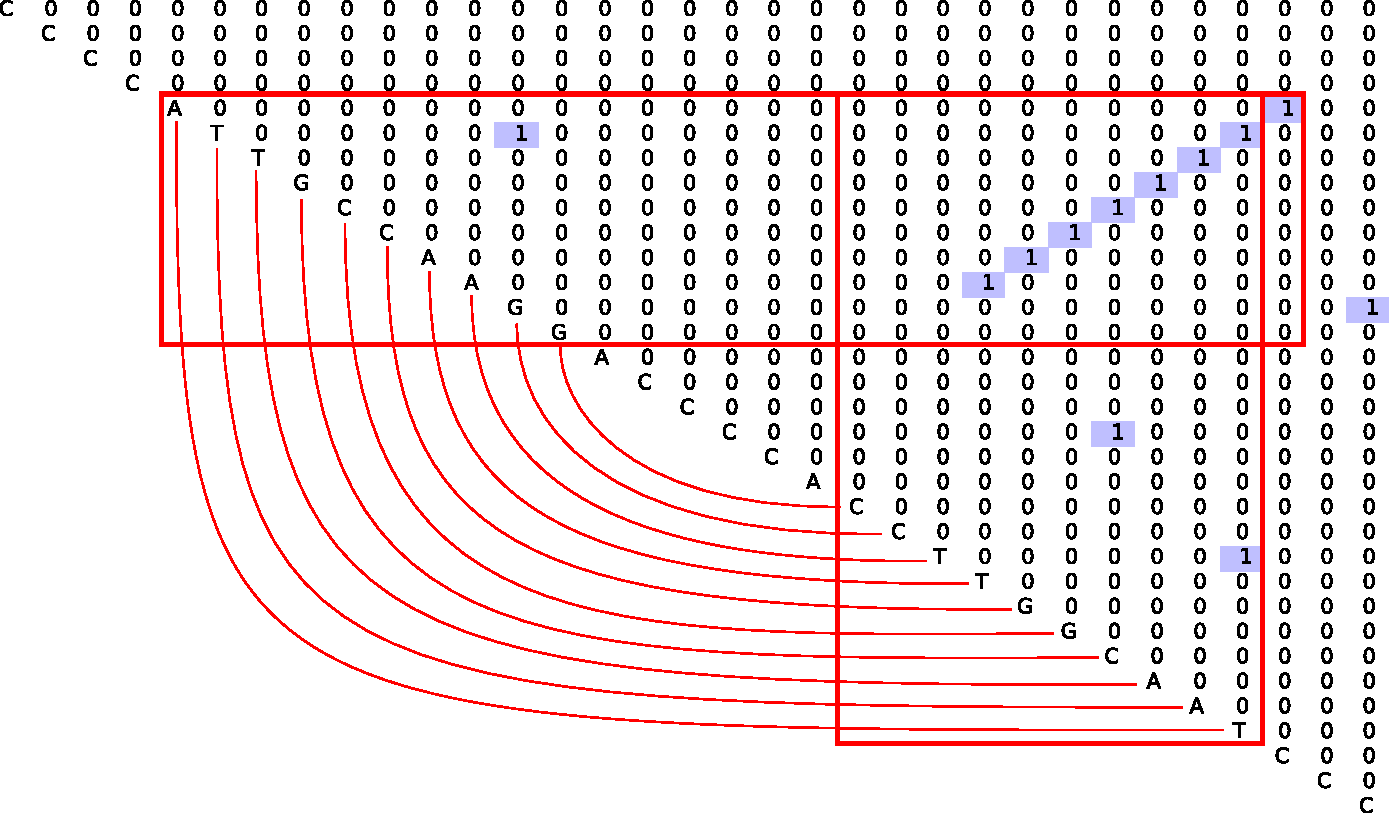
\includegraphics[width=0.8\textwidth]{figures/4.pdf}
\caption{Parsing result for sequence which should fold to
stem}
\label{fig:example}
\end{center}
\end{figure}

The parsing result in a form of a matrix can be linearized, compressed into a byte or int vector, and be further handled by a dense neural network, as described in~\cite{grigorevcomposition}.
Unfortunately, linearization breaks data locality: a diagonal chain of one-s, which signifies a high stem, is local in a matrix, but is broken apart during its linearization.
We see it to be an argument to investigate the applicability of convolutional networks for parsing result handling, as a boolean matrix can be converted to a black-white bitmap image.
In this paper, we provide an empirical comparison of networks which handle vectors and images.

Another problem is a bad performance of the earlier solution.
Since the trained network handles parsing result, each input sequence should first be parsed.
Parsing is a very time-consuming step: context-free parsing has cubic complexity in terms of the input length.
Even if we use matrix-based parsing algorithm~\cite{Azimov:2018:CPQ:3210259.3210264} which utilizes GPGPU, performance is insufficient.
We believe it would be better to avoid the parsing step at the final stage of the solution.
In this work, we propose a way to solve this problem by building a network which handles raw sequences, not parsing results.

\section{Convolution Neural Network Utilization}

First, we describe how to use a convolutional network for parsing result processing. Parsing result is a boolean matrix and we utilize the artificial neural network to detect sufficient features and find patterns in their appearance.
Therefore, we need to transform these boolean matrices to some data structure acceptable by the neural network: vector or image.
Currently, we came up with two possible ways.

The first one is to drop out the nullary bottom left triangle, vectorize the top right triangle row by row and transform it into a byte vector.
This approach reduces the input size, but it requires all the input sequences to have equal length.
Thus we propose to either cut sequences to be of some predefined length or to pad them up with some blank symbols.
Vectorization breaks data locality which makes learning harder: the network should restore back the relations broken during linearization.
This also means that learning takes more time.

The second way is to represent the matrix as an image: the false bits of the matrix as white pixels and the true bits as black ones.
This approach makes it possible to process sequences of different lengths since the images are easily transformed to a specified size.
Data locality is also preserved: the information about relative positions of extracted basic features does not get lost which should improve learning.

The architecture of the neural network that takes vectorized data as an input is described in~\cite{grigorevcomposition} and it consists of the long sequence of interchangeable dense and dropout layers with aggressive batch normalization. 
To handle images, we propose to use a network which consists of a small number of convolutional layers, linearization, and dense network which has a similar architecture as for vectorized data.
An example of proposed architecture id provided in figure~\ref{nn} (network \textbf{\texttt{N1}}).

\section{Parsing Step Elimination}

Another improvement that we came up with concerns parsing elimination in the context of our solution. 
The idea is to create a model which can handle original sequences instead of the parsing matrices. For that, we propose to use two-staged learning: first, a network which solves a subtask is trained and then it is used as pretrained layers in the training of the resulting network.
In our solution, we first train a neural network to handle parsing results which performs classification according to a problem at hands. We create two networks in order to compare different architectures: one of them handles vectorized parsing result, the other handles parsing result represented as a bitmap image. After that, we extend these neural networks by several input layers that take the initial nucleotide sequence as an input and convert it to the parsing result which is handled appropriately by the pretrained layers.

Figure~\ref{nn} represents the detailed description of these three neural networks architectures.
Here \textbf{\texttt{N1}} is a network which handles images, \textbf{\texttt{N2}} is a network which handles vectorized parsing results, and \textbf{\texttt{N0}} is an additional block which converts the input sequence into a set of features which can be handled by using \textbf{\texttt{N1}} or \textbf{\texttt{N2}}. So, firstly we train \textbf{\texttt{N1}} and \textbf{\texttt{N2}} on parsed data. After that, for vector-based network we combine the extension \textbf{\texttt{N0}} and the whole original sequence of layers and for image-based network we use the similar architecture, except we remove the convolutional layer from the extended model, thus, the first layer at the junction of the blocks corresponds to the linearized image.

\begin{figure}[h]
\begin{center}
\centering
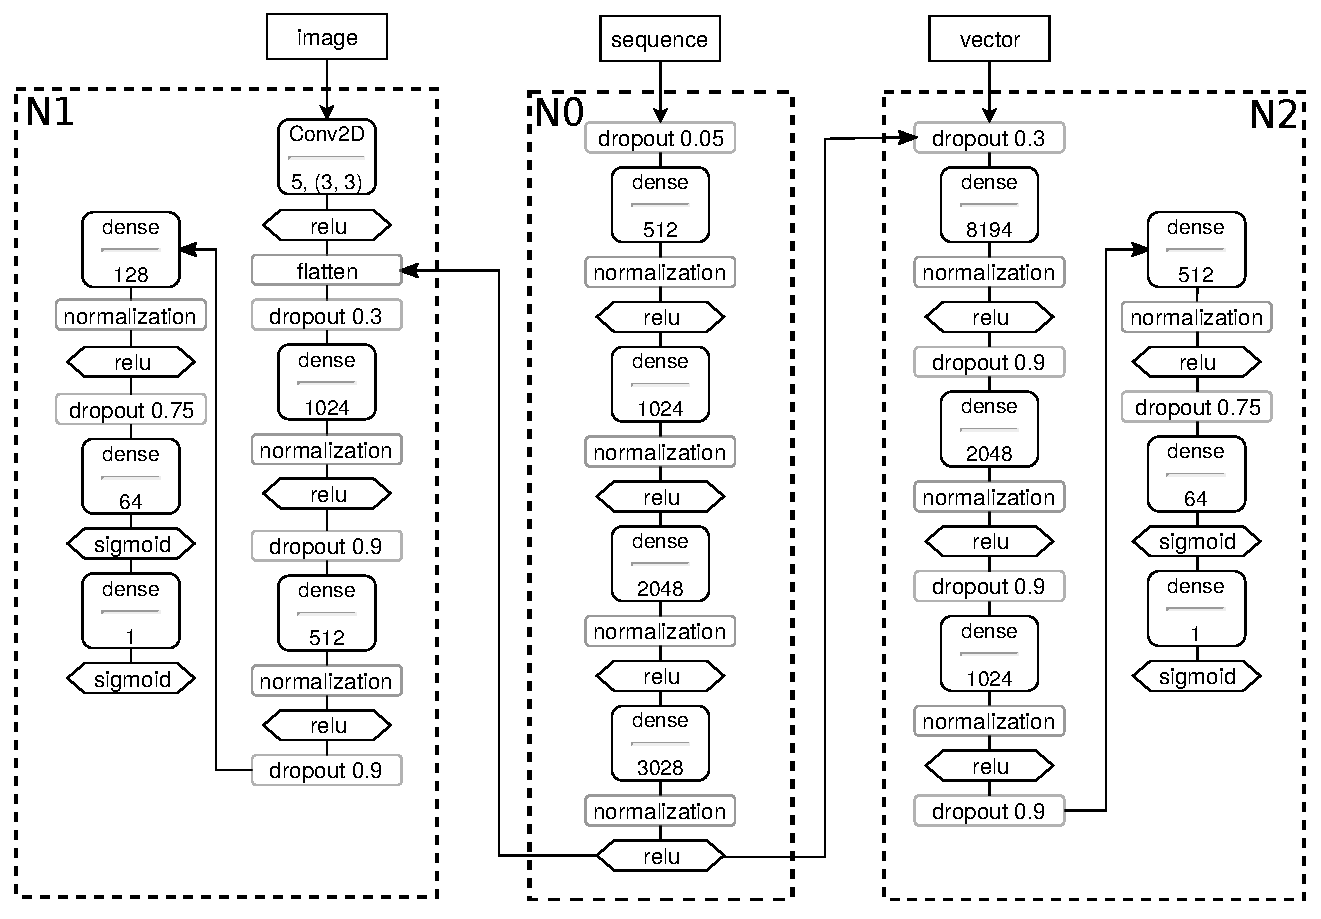
\includegraphics[width=12cm]{figures/nn_arch.pdf}
\caption{Neural networks architectures}
\label{nn}
\end{center}
\end{figure}

To sum up, we developed a technique to process parsing matrices as images by convolutional neural networks. 
Also, we built a model that handles sequences and requires parsing only for training the network it is based on. 
This removes the parsing step from the usage of the trained model.

In order to test the resulting solution we have implemented the frontend as a plugin using ReSharper SDK, so it can be installed into ReSharper, Rider and InspectCode.
The source code is parsed by internal ReSharper tools and the result is used to produce graphs and meta-information.
The issues found by the backend are shown using code highlighting.

The first analysis which has been implemented is the considered taint tracking analysis.
It is defined just by the PDA constructed in the section 2 translated into the code with some slight modifications which make it possible to process interactions with object fields.
To provide more information about an issue found by this analysis, the higlighting is accompanied by bulbs containing the full path of tainted variable from the source to the sink represented as the sequence of operations.

\subsection{Sample cases}

Let's look closer at properties of the resulting soluiton.
All these properties are illustrated by screenshots taken exactly from the runned Rider IDE with some small relocations of bulbs to make them not to overlap the code.

Firstly, the solution ensures flow sensitivity. I.e. it processes flow of variables passed into methods and returned from them correctly.
Which can be seen at fig~\ref{fig:ReturnsAndBrackets}.
This example illustrates the most common cases of interprocedural data passing.
\textit{Brackets} method gets the data, performs some computations on them and returns the result.
Invocations at lines 37 and 38 shows that the solution can distinguish two data flow paths despite both of them passes through the same method.
So, \textit{e} becomes tainted because \textit{c} is tainted and \textit{f} does not because \textit{d} is clear.
Moreover, the solution can track paths where passes and returns do not form the correct bracket sequence that is shown by method \textit{PostSource} which does not take any parameter and just returns tainted data.

\begin{figure}[h]
	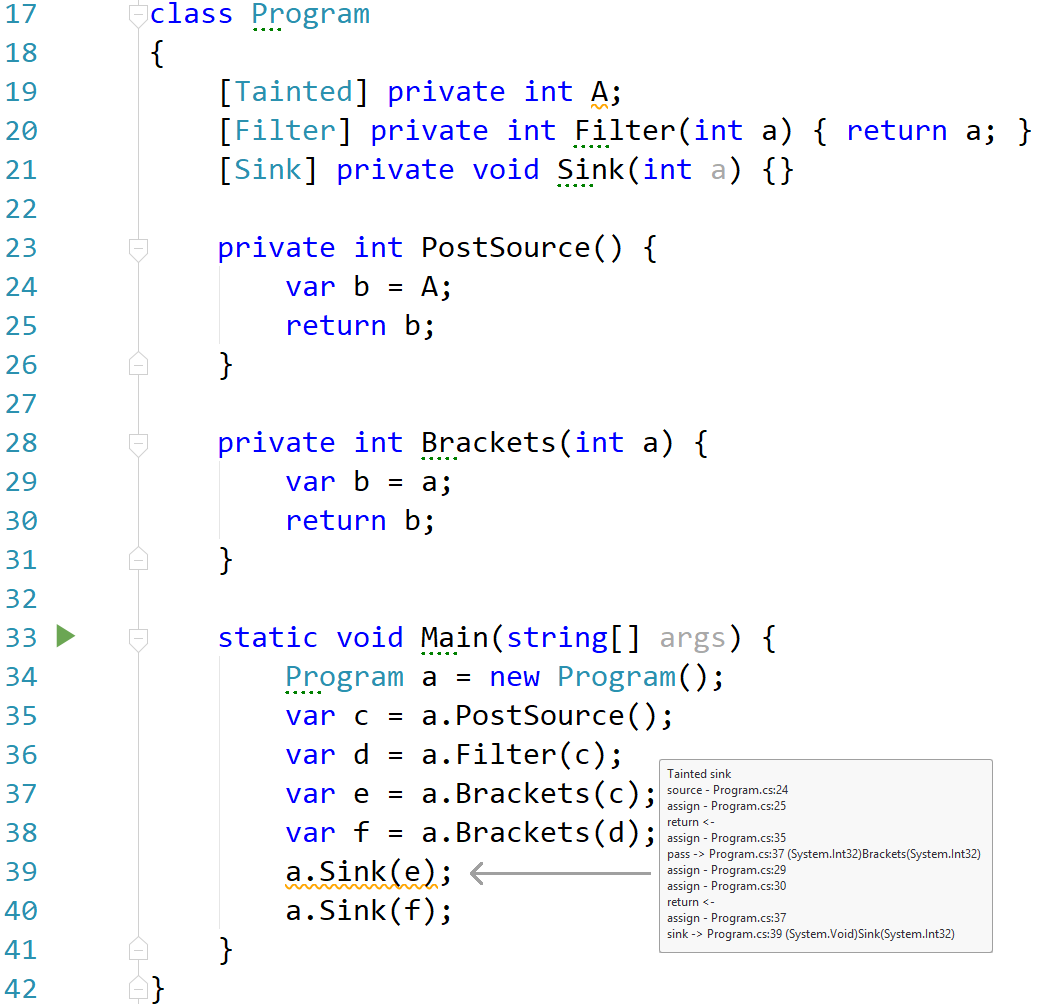
\includegraphics[width=\linewidth]{screenshots/ReturnsAndBrackets.png}
	\caption{Flow sensitivity}
	\label{fig:ReturnsAndBrackets}
\end{figure}

Secondly, the solution has the limited context sensitivity. I.e. it allows to track propagation of objects that are tainted by assigning of some fields inside them both by their own methods and by outer code interacting with their fields directly.
The first case is shown at fig~\ref{fig:ObjectTainting}.
There is the field \textit{B} at the line 18. 
This field can be used widely in the logic of the \textit{Container} class and by this the tainting of this field is considered as the tainting of the whole object.
However, while processing of the method \textit{Store} during the analysis it is hard to decide what the object need to be tainted because in the inner context of \textit{Store} it is just \textit{this} object.
I.e. we must consider the calling context to make such decision.
So, the solution provides this opportunity which is shown by lines 33-36 where the first invocation of \textit{Store} leads to the tainting of object \textit{d} and the second invocation does not taint object \textit{e}.

\begin{figure}[h]
	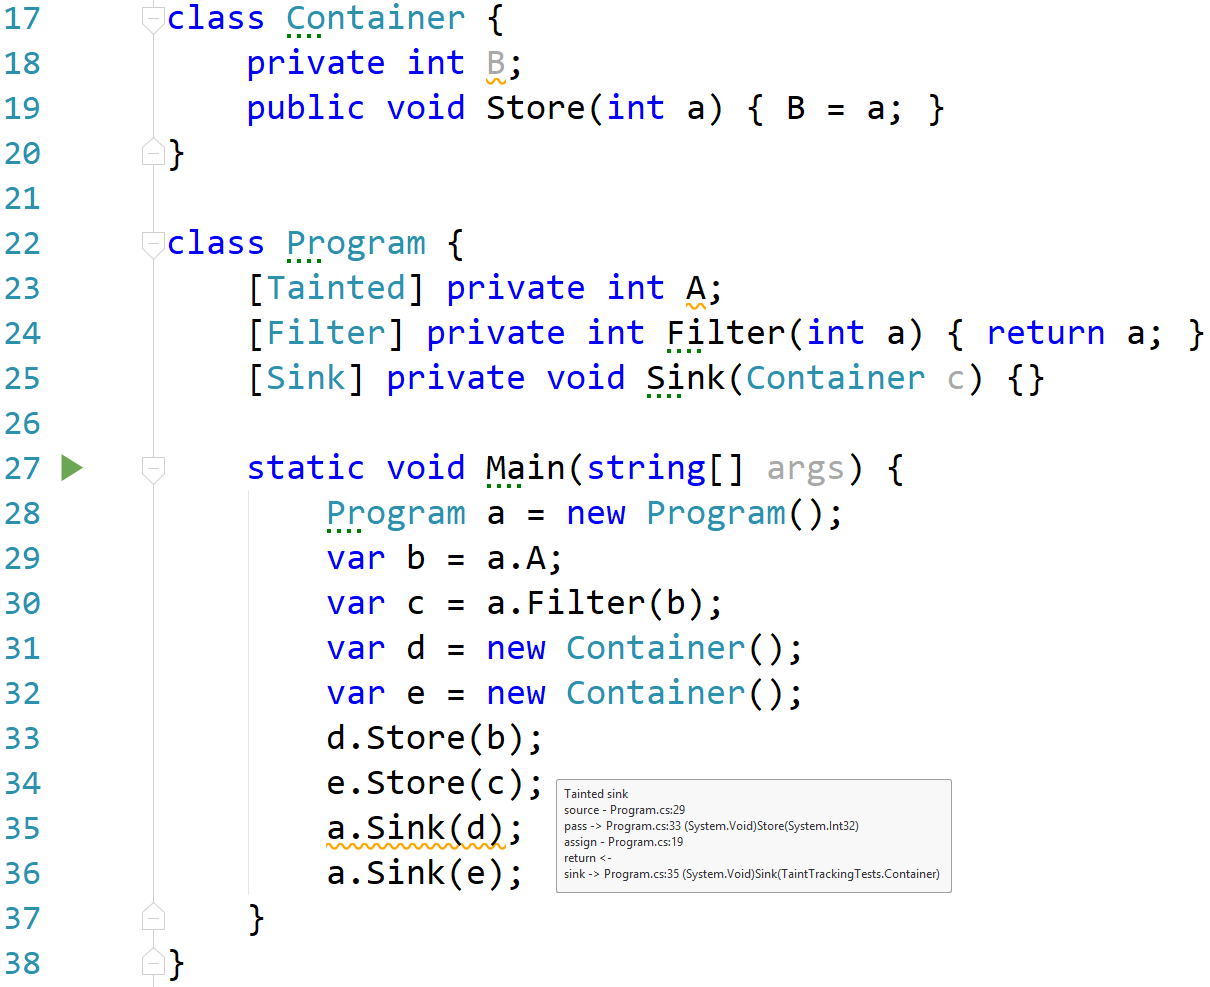
\includegraphics[width=\linewidth]{screenshots/ContextSensitivity.png}
	\caption{Tainting of an object by its own method}
	\label{fig:ObjectTainting}
\end{figure}

Finally, the solution works with any type of recursion and does not fall into infinite cycles.
It can be seen at fig.~\ref{fig:Recursion}.
This snippet contains two mutually recursive methods which pass the data to each other.
The solution checks all possible paths of passing even those which includes cyclic invocations and returns the passed variable to the point corresponding to the initial invocation.

\begin{figure}[h]
	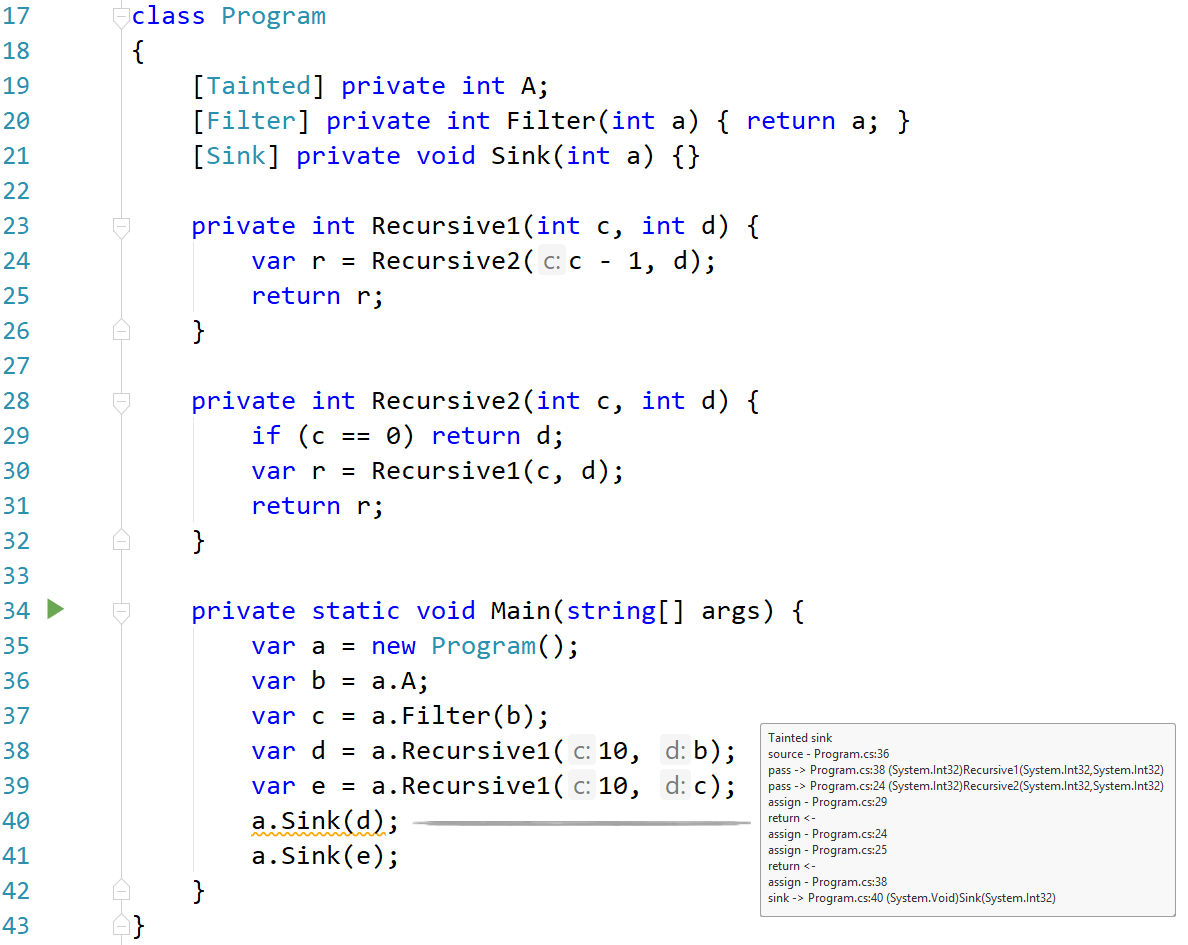
\includegraphics[width=\linewidth]{screenshots/Recursion.png}
	\caption{Recursive methods processing}
	\label{fig:Recursion}
\end{figure}

\subsection{Performance}

It is also necessary to measure the performance of the resulting solution.
Because the implemented taint tracking analysis forces to mark all participating entities manually, it is difficult to perform it on some large project.
However, there is another intermediate analysis which is runned before any other one to collect some information required by resolver.
In particular, it tracks propagation of all variables to discover all possible concrete types of each variable.
So, it involves each variable and each method in the whole program and thus the time and space required for execution of this analysis may be consistent estimation of the efficiency of the solution.

The code base that has been chosen as a source of data is the full solution of the Mono project.
(TODO: ADD SYSTEM CONFIGURATION).
The results is shown in the table~\ref{tab:Performance}.

\begin{table}[h]
	\begin{tabular}{|l|l|l|l|l|}
	\hline
		Project & Classes & Methods & \begin{tabular}[c]{@{}l@{}}Execution \\ time (s)\end{tabular} & \begin{tabular}[c]{@{}l@{}}Allocated \\ memory (GB)\end{tabular} \\ \hline
		Mono & 21013 & 192745 & $21\pm 0.5$ & $\sim 4.2$ \\ \hline
	\end{tabular}
	\caption{Performance}
	\label{tab:Performance}
\end{table}

\section{Conclusion}

We propose and implement in C\# programming language the generic framework for interprocedural static code analysis implementation.
This framework allows one to implement arbitrary interprocedural analysis in terms of CFL-reachability.
By using the proposed framework, we implement a plugin upon ReSharper infrastructure which provides simple taint analysis and demonstrate that our solution can handle important real-world cases.
Also we show that the proposed framework can be used for real-world solutions analysis.

One of the directions for future work is a creation of analysis and its evaluation on real-world projects.
By this way, we want to get information which helps to improve the usability of our framework: tune performance, improve API, etc.
Also we should improve documentation and create more examples of usage.

Another direction is a practical evaluation of automatic fix location prediction by using minimum cuts method~\cite{10.1007/978-3-319-63390-9_27}.

Also we want to compare the proposed approach with other generic CFL-reachability based approaches for interprocedural code analysis cretion. For example, fith generation-based approach~\cite{LPAR-21:Cauliflower_Solver_Generator_for}, which idea is similar to parser generators.


%
% ---- Bibliography ----
%
% BibTeX users should specify bibliography style 'splncs04'.
% References will then be sorted and formatted in the correct style.
%
\bibliographystyle{splncs04}
\bibliography{main}

\end{document}

